\chapter{Design Principles \& Design Patterns}
\label{ch:design}

Good design is not about cleverness; it is about managing complexity so that future changes are cheap and safe. This chapter introduces the principles that guide object-oriented design and the classic Gang-of-Four (GoF) patterns that reify those principles into reusable solutions.

\section{Why Design Matters}

Code has two audiences: the machine and the next developer. Design quality shows up in change cost. A well-designed system absorbs a new requirement with a small, localised edit; a poorly designed one requires shotgun surgery across dozens of files. Two metrics predict this:

\begin{itemize}
    \item \textbf{Coupling} --- degree of interdependence between modules. Lower is better.
    \item \textbf{Cohesion} --- how closely the responsibilities within a module belong together. Higher is better.
\end{itemize}

\begin{figure}[h]
\centering
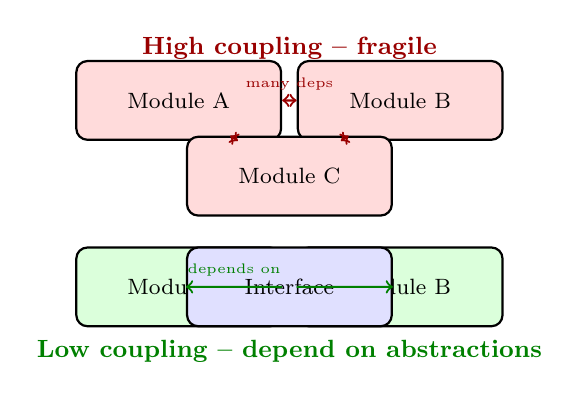
\begin{tikzpicture}[scale=0.74, every node/.style={font=\footnotesize}]
  \tikzstyle{mod}=[draw,rounded corners,minimum width=2.6cm,minimum height=1.0cm,align=center,thick]
  % High coupling bad
  \node[mod,fill=red!14] (a1) at (0,2.2) {Module A};
  \node[mod,fill=red!14] (b1) at (3.8,2.2) {Module B};
  \node[mod,fill=red!14] (c1) at (1.9,0.9) {Module C};
  \draw[<->,thick,red!60!black] (a1) -- (b1) node[midway,above,font=\tiny] {many deps};
  \draw[<->,thick,red!60!black] (a1) -- (c1);
  \draw[<->,thick,red!60!black] (b1) -- (c1);
  \node[font=\small\bfseries,red!60!black] at (1.9,3.1) {High coupling -- fragile};
  % Low coupling good
  \node[mod,fill=green!14] (a2) at (0,-1.0) {Module A};
  \node[mod,fill=green!14] (b2) at (3.8,-1.0) {Module B};
  \node[mod,fill=blue!12] (iface) at (1.9,-1.0) {Interface};
  \draw[->,thick,green!50!black] (a2) -- (iface) node[midway,above,font=\tiny] {depends on};
  \draw[->,thick,green!50!black] (b2) -- (iface);
  \node[font=\small\bfseries,green!50!black] at (1.9,-2.1) {Low coupling -- depend on abstractions};
\end{tikzpicture}
\caption{Coupling contrast: dense mutual dependencies (top, fragile) versus dependency on a shared abstraction (bottom, stable). Cohesion is high when each module has one focused responsibility.}
\end{figure}

Common coupling types from worst to best: content $>$ common $>$ external $>$ control $>$ stamp $>$ data $>$ message $>$ no coupling. Cohesion levels from worst to best: coincidental $<$ logical $<$ temporal $<$ procedural $<$ communicational $<$ sequential $<$ functional (goal).

\section{SOLID Principles}

SOLID (Martin, 2000) distils five design rules for maintainable OO systems:

\subsection{Single Responsibility Principle (SRP)}

A class should have one, and only one, reason to change. If a class handles both business logic and persistence, a database migration forces a change to business code. Split them.

\subsection{Open/Closed Principle (OCP)}

Software entities should be \emph{open for extension, closed for modification}. Add new behaviour by adding new code, not by editing existing code. Achieved via abstraction and polymorphism.

\subsection{Liskov Substitution Principle (LSP)}

Subtypes must be substitutable for their base types without breaking correctness. If \texttt{Square} extends \texttt{Rectangle} but violates the invariant that width and height are independent, LSP is broken.

\subsection{Interface Segregation Principle (ISP)}

Clients should not be forced to depend on interfaces they do not use. Prefer several small, focused interfaces over one fat interface.

\subsection{Dependency Inversion Principle (DIP)}

High-level modules should not depend on low-level modules; both should depend on abstractions. This is the ``D'' that enables testability via mocking.

\begin{figure}[h]
\centering
\begin{tikzpicture}[scale=0.72, every node/.style={font=\scriptsize}]
  \tikzstyle{cls}=[draw,rounded corners,minimum width=2.8cm,minimum height=0.85cm,align=center,thick]
  % Without DIP -- bad
  \node[cls,fill=red!12] (hl1) at (0,1.8) {High-level: ReportService};
  \node[cls,fill=red!12] (ll1) at (0,0.4) {Low-level: MySQLStore};
  \draw[->,thick,red!60!black] (hl1) -- (ll1) node[midway,right,font=\tiny] {direct dep.};
  \node[font=\tiny,red!60!black] at (0,-0.35) {Brittle: change DB $\to$ change service};
  % With DIP -- good
  \node[cls,fill=green!14] (hl2) at (5.5,1.8) {ReportService};
  \node[cls,fill=blue!12] (abs) at (5.5,0.4) {\textit{<<interface>>} DataStore};
  \node[cls,fill=orange!14] (ll2) at (5.5,-0.9) {MySQLStore};
  \draw[->,thick,green!50!black] (hl2) -- (abs);
  \draw[->,thick,dashed] (ll2) -- (abs) node[midway,right,font=\tiny] {implements};
  \draw[-{Triangle[open,length=3mm]},thick,gray] (ll2.north) -- (abs.south);
  \node[font=\tiny,green!50!black] at (5.5,-1.65) {Stable: swap store without touching service};
  \node[font=\small\bfseries] at (2.75,2.7) {DIP: depend on abstractions};
\end{tikzpicture}
\caption{Dependency Inversion: before (left, high-level depends on low-level) versus after (right, both depend on an abstraction). The right side enables testing with a fake store.}
\end{figure}


\section{GRASP -- Assigning Responsibilities}

General Responsibility Assignment Software Patterns (GRASP) complement SOLID with heuristics for assigning responsibilities to classes: \emph{Information Expert} (assign to the class that has the data), \emph{Creator} (who should create an object), \emph{Controller} (first object beyond the UI that handles system events), \emph{Low Coupling / High Cohesion}, \emph{Polymorphism}, \emph{Pure Fabrication} (invent a class to achieve low coupling when no domain class fits), \emph{Indirection}, and \emph{Protected Variations}. GRASP is especially useful when drawing sequence diagrams: each message assignment can be justified by a GRASP principle.

\section{Gang-of-Four Design Patterns}

Patterns are proven solutions to recurring design problems. The GoF catalogue has 23~patterns in three families: creational, structural, behavioural. We cover four essentials.

\subsection{Singleton (Creational)}

Ensures a class has exactly one instance and provides global access. Classic use: configuration manager, logger, connection pool.

\begin{lstlisting}[language=Java,caption={Thread-safe Singleton (double-checked locking).}]
public final class Config {
    private static volatile Config instance;
    private Config() {} // prevent external instantiation
    public static Config getInstance() {
        if (instance == null) {
            synchronized (Config.class) {
                if (instance == null) instance = new Config();
            }
        }
        return instance;
    }
}
\end{lstlisting}

Caution: singletons hide dependencies and complicate testing. Prefer dependency injection when possible; use singleton only when single-instance semantics are truly required.

\subsection{Factory Method / Simple Factory (Creational)}

Encapsulates object creation so clients depend on an abstraction, not concrete classes. Adding a new product type requires only a new subclass, satisfying OCP.

\begin{lstlisting}[language=Java,caption={Factory Method -- creation delegated to subclasses.}]
abstract class DocumentFactory {
    abstract Document createDocument();
}
class PdfFactory extends DocumentFactory {
    Document createDocument() { return new PdfDocument(); }
}
class WordFactory extends DocumentFactory {
    Document createDocument() { return new WordDocument(); }
}
// Client code
DocumentFactory f = new PdfFactory();
Document doc = f.createDocument(); // no 'new PdfDocument()' in client
\end{lstlisting}

\subsection{Observer (Behavioural)}

Defines a one-to-many dependency: when the subject changes state, all observers are notified automatically. Foundation of MVC, event buses, and reactive UI.

\begin{figure}[h]
\centering
\begin{tikzpicture}[scale=0.74, every node/.style={font=\scriptsize}]
  \tikzstyle{cls}=[draw,rounded corners,minimum width=2.7cm,minimum height=0.9cm,align=center,thick]
  \node[cls,fill=blue!14] (subj) at (0,2.0) {\textbf{Subject}\\\rule{2.4cm}{0.4pt}\\ \texttt{+attach(o: Observer)}\\ \texttt{+notify()}};
  \node[cls,fill=green!14] (obs) at (5.5,2.0) {\textbf{Observer}\\\rule{2.4cm}{0.4pt}\\ \textit{+update()}};
  \node[cls,fill=orange!14] (concS) at (0,0.3) {ConcreteSubject\\\texttt{-state}};
  \node[cls,fill=violet!14] (concO) at (5.5,0.3) {ConcreteObserver};
  \draw[-{Triangle[open,length=3mm]},thick] (concS.north) -- (subj.south);
  \draw[-{Triangle[open,length=3mm]},thick] (concO.north) -- (obs.south);
  \draw[->,thick,blue!60!black] (concS) -- (concO) node[midway,above,font=\tiny,align=center] {notifies\\(loop over observers)};
  \node[font=\tiny,gray] at (2.75,1.2) {1 -- *};
  \draw[thick,gray] (subj.east) -- (obs.west);
\end{tikzpicture}
\caption{Observer pattern structure -- subject maintains a list of observers and notifies them on state change. Decouples subject from concrete observer types.}
\end{figure}

\subsection{Strategy (Behavioural)}

Encapsulates interchangeable algorithms behind a common interface so the algorithm can vary independently of clients. Eliminates conditional chains (\texttt{if type==A ... else if type==B}).

\begin{lstlisting}[language=Java,caption={Strategy -- interchangeable payment algorithms.}]
interface PaymentStrategy { void pay(int amount); }
class CreditCardPayment implements PaymentStrategy {
    public void pay(int amount) { /* charge card */ }
}
class PayNowPayment implements PaymentStrategy {
    public void pay(int amount) { /* PayNow transfer */ }
}
class Checkout {
    private PaymentStrategy strategy;
    Checkout(PaymentStrategy s) { this.strategy = s; }
    void complete(int amount) { strategy.pay(amount); }
}
\end{lstlisting}

Choosing a pattern: use Factory when creation logic is complex or varies; Observer when one state change must propagate to many dependents; Strategy when you have a family of algorithms selected at runtime; Singleton sparingly, when global single-instance semantics are essential.


\section{Package Design and Metrics}

Beyond class-level principles, package-level design governs large systems. Three package principles mirror SOLID at a higher scale: \emph{Reuse--Release Equivalence} (reused packages must be released as units), \emph{Common Closure} (classes that change together belong together), and \emph{Common Reuse} (classes that are not reused together should not be packaged together). Metrics such as efferent/afferent coupling ($C_e$, $C_a$) and instability $I = C_e/(C_a+C_e)$ quantify package coupling; distance from the main sequence $D = |A + I - 1|$ (where $A$ is abstractness) flags packages that are either too concrete and unstable or too abstract and stable.

\section{Exercises}

\begin{exercise}
A class \texttt{ReportGenerator} formats reports, fetches data from MySQL, and sends emails. Identify the SRP violation, refactor into three classes, and draw the resulting class diagram with dependencies.
\end{exercise}

\begin{exercise}
Show how Strategy satisfies OCP: start with a \texttt{DiscountCalculator} using \texttt{if-else} on customer type, then refactor to Strategy. How does adding a new customer type differ before and after?
\end{exercise}

\begin{exercise}
Implement Observer for a stock ticker where multiple displays (price chart, alert panel, log) update when the price changes. Explain why push vs.\ pull notification matters for performance when updates are frequent.
\end{exercise}

\begin{exercise}
A developer makes every service class a Singleton ``for convenience.'' Give two concrete harms this causes for unit testing and concurrency, and propose an alternative using dependency injection.
\end{exercise}

\begin{exercise}
Compare Factory Method and Abstract Factory. When would you choose one over the other? Illustrate with a UI toolkit that must support both Light and Dark themes across Button and Menu families.
\end{exercise}
